%%%%%%%%%%%%%%%%%%%%%%%%%%%%%%%%%%%%%%%%%%%%%%%%%%%%%%%%%%%%%%%%%%%%%%%%%%%%%%%%
% Uncertainties and Results:
%%%%%%%%%%%%%%%%%%%%%%%%%%%%%%%%%%%%%%%%%%%%%%%%%%%%%%%%%%%%%%%%%%%%%%%%%%%%%%%%
\chapter{Statistical Analysis, Uncertainties, and Results}
\label{statAnalysis_uncerts_results}
%%%%%%%%%%%%%%%%%%%%%%%%%%%%%%%%%%%%%%%%%%%%%%%%%%%%%%%%%%%%%%%%%%%%%%%%%%%%%%%%
The selections described in Chapter \ref{sec:event_selection_chapter} were applied to data, backgrounds 
and simulated \WR signals, and 
the selected events were used to produce $\Mlljj$ distributions in the $ee$- and $\mu\mu$-channels.  
Each $\Mlljj$ distribution ($\Mlljj > 600$ $\GeV$) was divided into smaller $\Mlljj$ windows linked 
to specific \mWR hypotheses.  The size of each window was optimized by calculating cross section $\times$ 
branching fraction limits with Bayesian statistics.


%%%%%%%%%%%%%%%%%%%%%%%%%%%%%%%%%%%%%%%%%%%%%%%%%%%%%%%%%%%%%%%%%%%%%%%%%%%%%%%%
% Statistical Analysis 
%%%%%%%%%%%%%%%%%%%%%%%%%%%%%%%%%%%%%%%%%%%%%%%%%%%%%%%%%%%%%%%%%%%%%%%%%%%%%%%%
\section{Statistical Analysis}
\label{sec:statAnalysis}
%%%%%%%%%%%%%%%%%%%%%%%%%%%%%%%%%%%%%%%%%%%%%%%%%%%%%%%%%%%%%%%%%%%%%%%%%%%%%%%%
\subsection{Bayesian Limits}
\label{sec:bayesianStatsAndLimits}
Generic cross section $\times$ branching fraction limits are calculated using several quantities 
obtained after all selections were applied: the 
number of measured events $G$, the estimated number of signal events $S$ and background events $B$, 
and the signal and background event uncertainties $\delta S$ and $\delta B$.  In the \WR search, 
limits on $\sigma(\WR) \times BR(\WR \rightarrow \ell\ell jj)$ were calculated in two scenarios: 
``expected'' limits where $G = B$, and ``observed'' limits, the results, where $G$ equaled the number 
of selected events in data.  Expected limits were calculated to optimize the sizes of $\Mlljj$ windows, 
in which the observed limits were calculated to test different \mWR hypotheses.  In both scenarios 
limits were calculated at 95\% confidence level (CL) using a Poisson model of the $S \plus B$ events:

\begin{equation}
	Poisson(\mu S(\pmb{\theta}) \thickspace \plus \thickspace B(\pmb{\theta}))
	\label{eq:poissonModel}
\end{equation}
where $\mu$ was the unknown, dimensionless \WR signal strength, and $\pmb{\theta}$ represented the uncertainties $\delta S$ 
and $\delta B$ described later in Section \ref{sec:uncertainties}.  Using Bayesian statistics, the probability 
distribution for $\mu$ given $G$ measured events, $p(\mu|G)$, was obtained by evaluating the integral\cite{bayesianDataAnalysis}:

\begin{equation}
	p(\mu|G) = \int p(\mu|\pmb{\theta},G)p(\pmb{\theta}|G)d\pmb{\theta}
	\label{eq:sigStrngthProbDist}
\end{equation}
where $p(\pmb{\theta}|G)$ were the probability distributions for the uncertainties given the measurement 
$G$ (``marginal posterior distributions''), and $p(\mu|\pmb{\theta},G)$ were the probability distributions 
for $\mu$ given the uncertainties, and the measurement $G$ (``conditional posterior distributions'').  
Functional forms of the marginal posterior distributions were either log-normal or Gamma distributions 
depending on the uncertainty, and are identified later in Section \ref{sec:uncertainties}.  Functional forms 
of the conditional posterior distributions were derived from uniform prior distributions and Equation 
\ref{eq:poissonModel}.  The integrals in Equation \ref{eq:sigStrngthProbDist} were evaluated 
numerically using \MC simulations to obtain $p(\mu|G)$.  Then, $p(\mu|G)$ was integrated from $\mu =$ 0 
to $\mu = \mu_{max}$ such that 95\% of the area under $p(\mu|G)$ was covered.  The value $\mu_{max}$ was the 
95\% CL upper limit on the signal strength; and $\mu_{max}$ was multiplied by $\sigma(\WR)$ obtained from 
\WR simulations to calculate a limit on $\sigma(\WR) \times BR(\WR \rightarrow \ell\ell jj)$.

\subsection{$\Mlljj$ Windows}
\label{sec:mlljjWindows}
The difference in the $\Mlljj$ distribution shape between selected ST background and simulated \WR events motivated the 
use of finite size $\Mlljj$ windows to search for evidence of different \mWR hypotheses.  A \WR signal appeared as a 
peak in the $\Mlljj$ distribution, with tails above and below the peak that grew longer with increasing \mWR, 
as shown in Figure \ref{fig:signalShapesAfterSelection}.  In contrast, the $\Mlljj$ distribution found in all ST 
backgrounds decreased rapidly with increasing $\Mlljj$.  To transform this difference in the $\Mlljj$ shape into 
greater signal over background sensitivity, the $\Mlljj > 600$ $\GeV$ range was divided into smaller $\Mlljj$ 
windows linked to specific \mWR hypotheses.  The size of each $\Mlljj$ window was optimized for its corresponding 
\mWR hypothesis using the following procedure:

\begin{itemize}
	\item $\sim$150 $\Mlljj$ windows of different sizes were defined based on the width of the simulated \WR $\Mlljj$ distribution.
	\item In each window:
	\begin{itemize}
		\item The number of signal events $S$ and background events $B$ were counted.
		\item A Poisson distribution was made with mean equal to $B$, and a random number $C$ was pulled 
			from the Poisson distribution that represented the number of measured events in the window.
		\item Using the procedure described in Section \ref{sec:bayesianStatsAndLimits}, an expected 
			upper limit on $\sigma(\WR) \times BR(\WR \rightarrow \ell\ell jj)$ at 95\% CL was calculated 
			based on the probability of measuring $C$ due to fluctuations in $S$ and $B$.  To expedite the calculation, 
			only statistical uncertainties were considered in the fluctuations of $S$ and $B$.
		\item The expected limit was recalculated 300 times, and each time a new random number $C$ was 
			pulled from the Poisson distribution with mean $B$.  The expected upper limit for the window 
			was the median value of all 300 limits.
	\end{itemize}
	\item The optimized window was chosen as the window that minimized the expected upper limit.
\end{itemize}

\begin{figure}[btp]
	\centering
	\subfigure{
		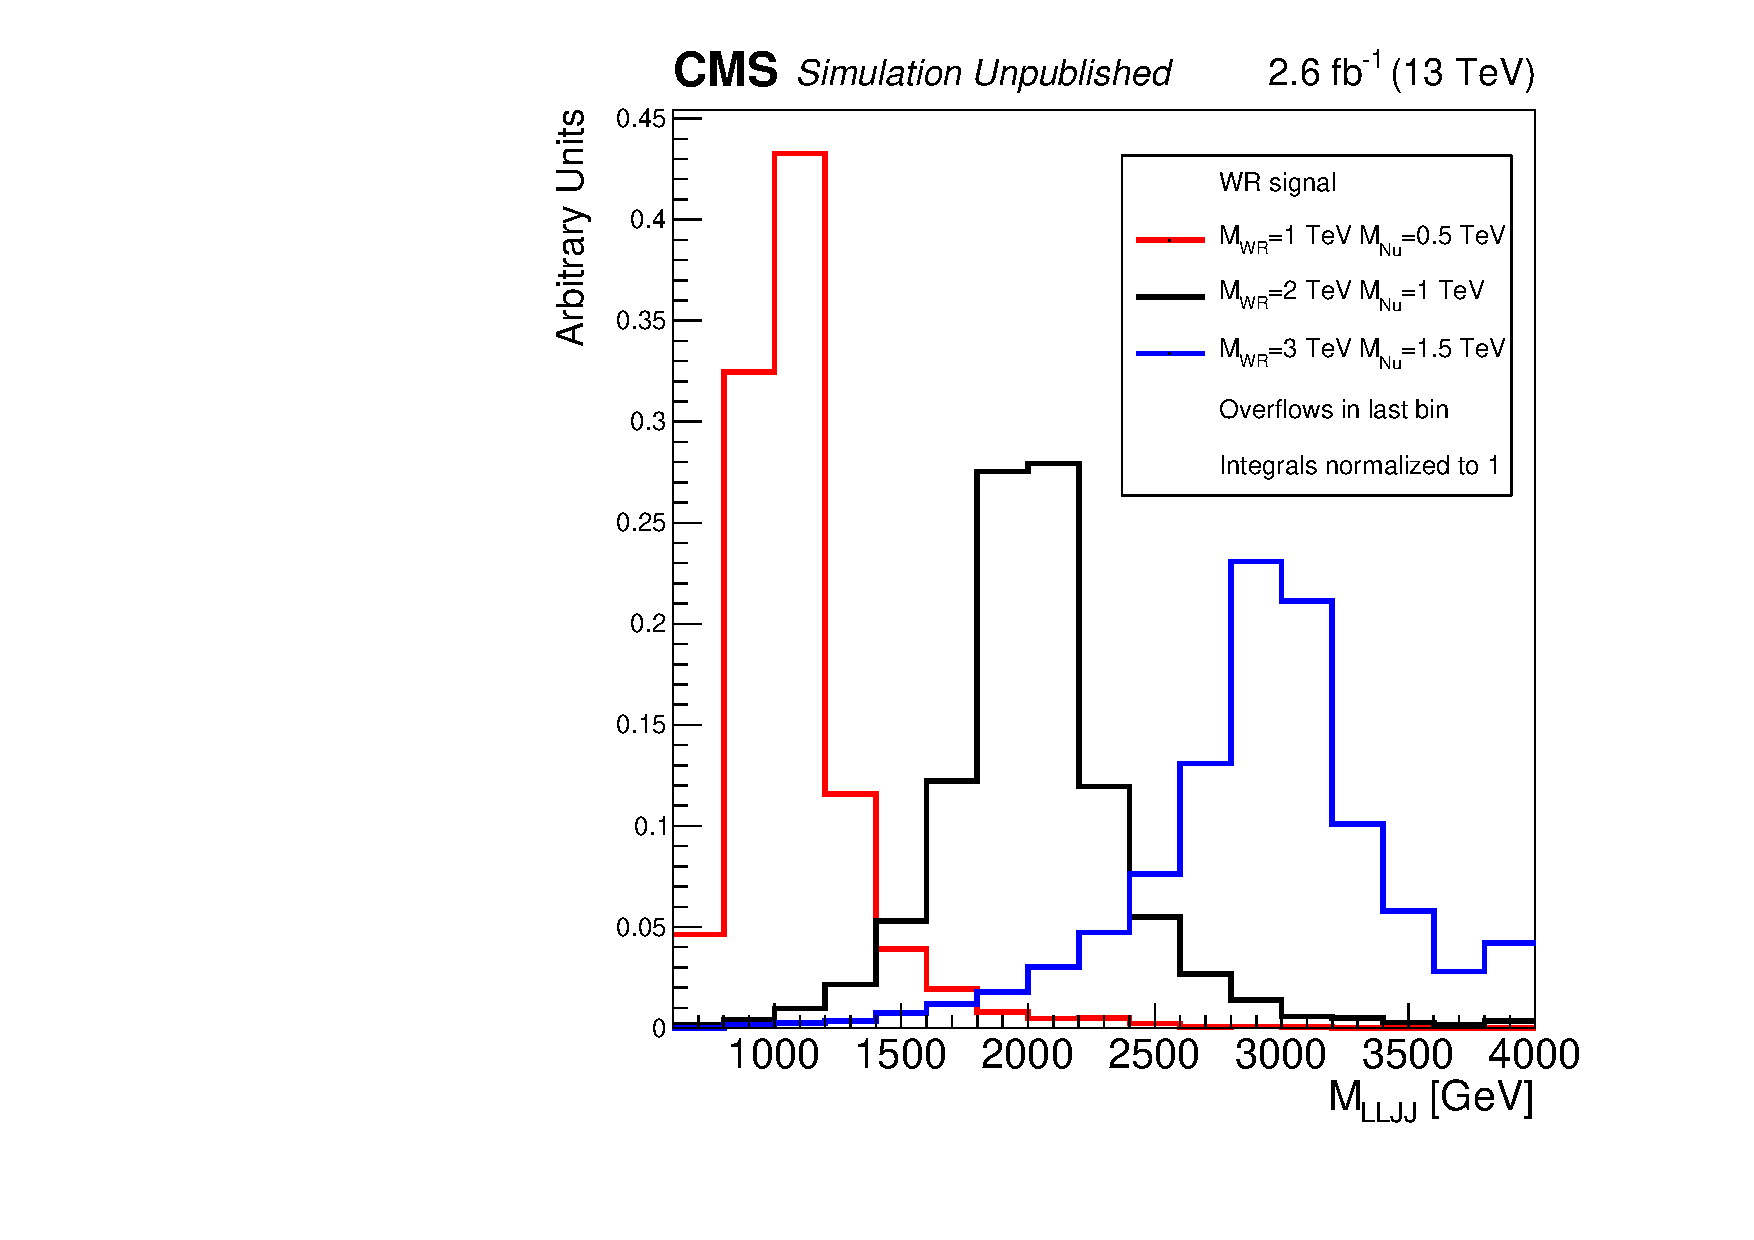
\includegraphics[width=0.65\textwidth]{figures/Mlljj_signalRegionCuts_severalWrSignals_EE.pdf}
	}
	\subfigure{
		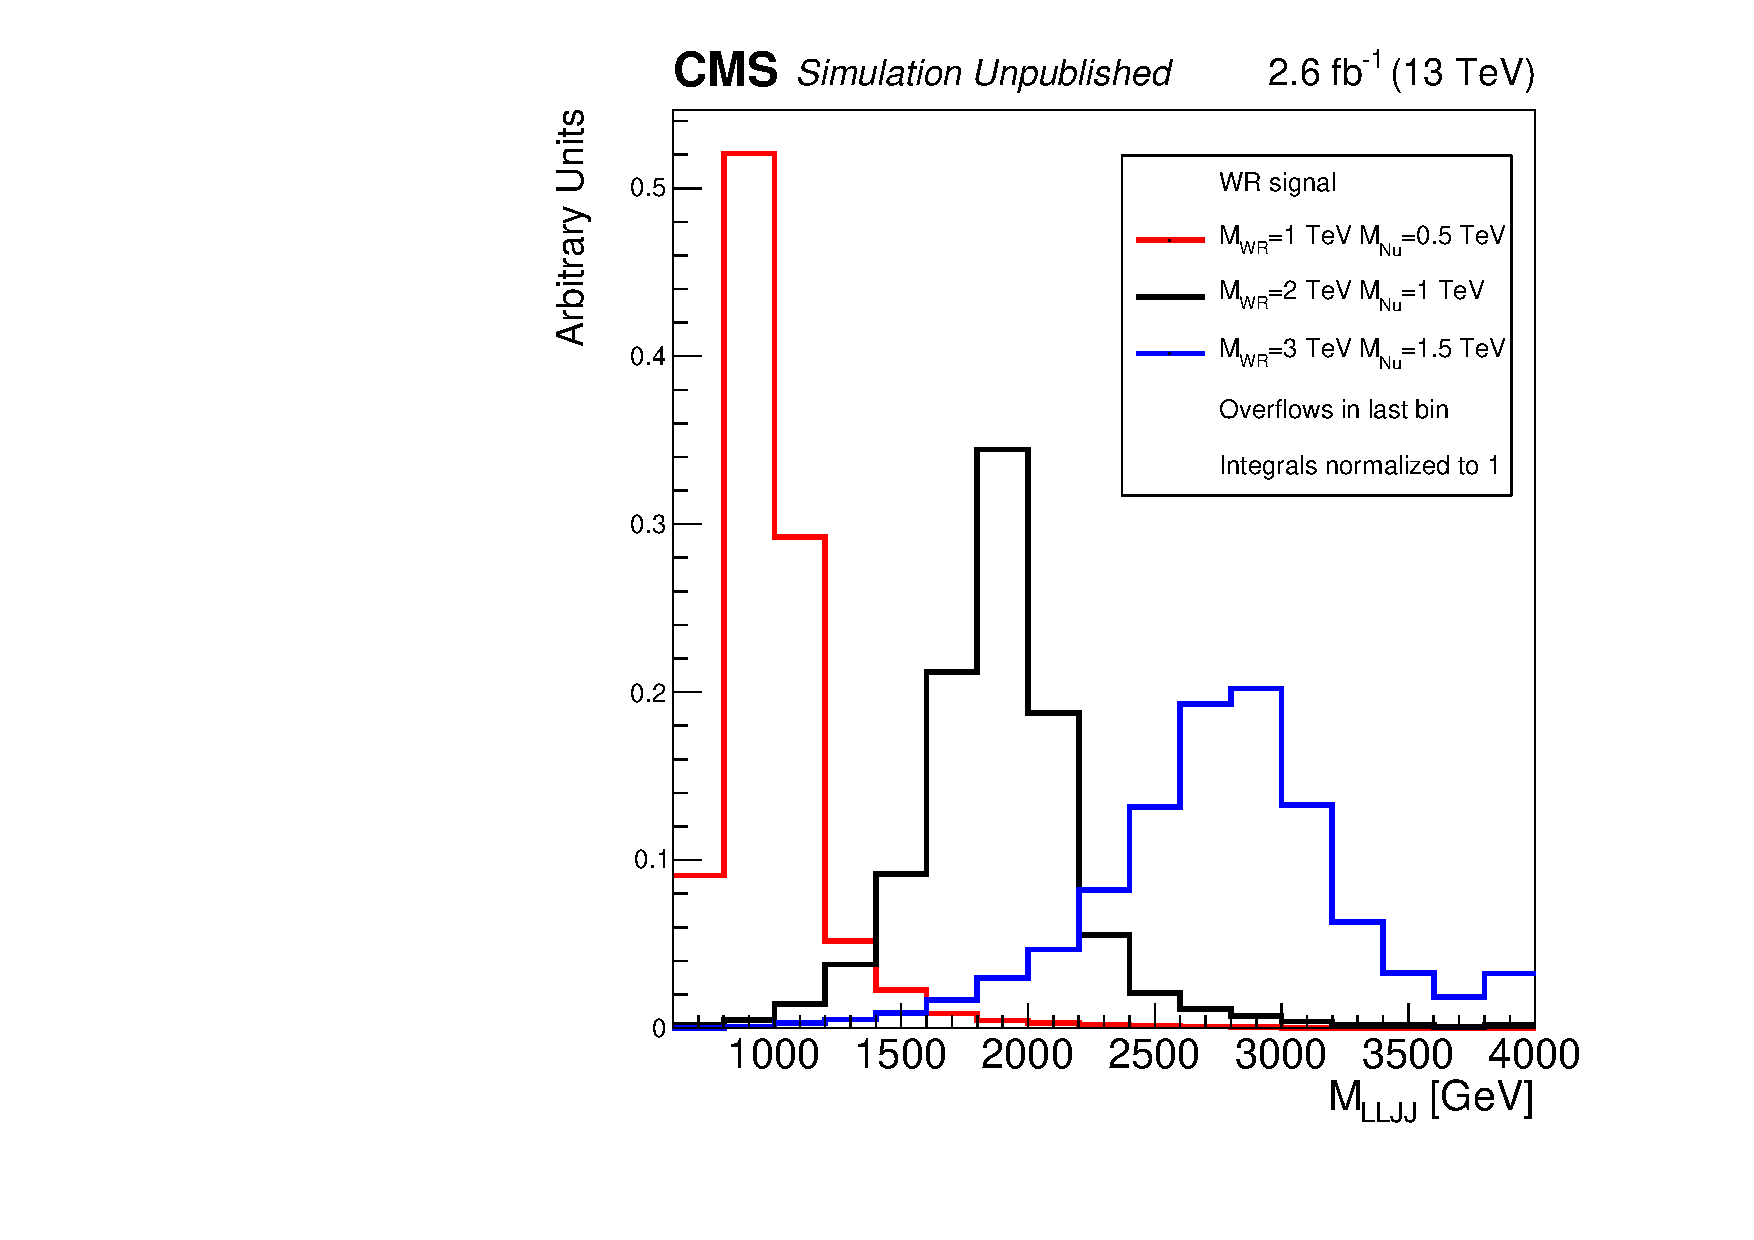
\includegraphics[width=0.65\textwidth]{figures/Mlljj_signalRegionCuts_severalWrSignals_MuMu.pdf}
	}
	\label{fig:signalShapesAfterSelection}
	\caption{The $\Mlljj$ distribution after all selections using simulated \WR signal events with several \mWR hypotheses.  The 
	$ee$- ($\mu\mu$-) channel is shown on the left (right).}
\end{figure}

The optimized windows, listed in Table \ref{tab:masscuts}, overlapped in $\Mlljj$ because any selected event could be 
consistent with several \mWR hypotheses.  In each window the number of data events, $\DY$ and top quark background events, 
and simulated \WR events\footnote{In the window optimized for $\mWR = 1000$ $\GeV$, only events produced in the $\mWR = 1000$ $\GeV$ 
simulation were counted.} were counted, and were used to calculate observed and expected upper limits on 
$\sigma(\WR) \times BR(\WR \rightarrow \ell\ell jj)$.

\begin{table}[h]
\caption{$\Mlljj$ window ranges that minimized the expected upper limit on the \WR cross section at different \mWR values.}
\label{tab:masscuts}
\centering
\begin{tabular}{|c|r@{ - }l|r@{ - }l|} \hline
\mWR (\GeV) & \multicolumn{4}{c|}{\Mlljj window (\GeV)}  \\\hline
& \multicolumn{2}{c|}{Electrons}  & \multicolumn{2}{c|}{Muons}  \\  \hline
 800  & 700       &  1100       &  700       &  1200      \\  \hline
1000  & 900       &  1300       &  900       &  1400      \\  \hline
1200  & 1100       &  1550       &  1100       &  1650      \\  \hline
1400  & 1250       &  1750       &  1300       &  1850      \\  \hline
1600  & 1450      &  2000       &  1500      &  2100      \\  \hline
1800  & 1600      &  2250       &  1600      &  2300      \\  \hline
2000  & 1850      &  2550       &  1850      &  2600      \\  \hline
2200  & 2000      &  2800       &  2000      &  2850      \\  \hline
2400  & 2150      &  3100       &  2150      &  3100      \\  \hline
2600  & 2250      &  3400       &  2300      &  3400      \\  \hline
2800  & 2350      &  3700       &  2400      &  3700      \\  \hline
3000  & 2500      &  4000       &  2500      &  3950      \\  \hline
3200  & 2550      &  4300       &  2700      &  4250      \\  \hline
3600  & 2700      &  4900       &  2900      &  4850      \\  \hline
3800  & 2750      &  5200       &  2950      &  5150      \\  \hline
4000  & 2800      &  5500       &  3000      &  5450      \\  \hline
4200  & 2800      &  5750       &  3100      &  5750      \\  \hline
4400  & 2850      &  6050       &  3150      &  6100      \\  \hline
4600  & 2850      &  6300       &  3150      &  6400      \\  \hline
4800  & 2850      &  6600       &  3200      &  6700      \\  \hline
5000  & 2900      &  6850       &  3200      &  7000      \\  \hline
5200  & 2900      &  7050       &  3200      &  7300      \\  \hline
5600  & 2900      &  7500       &  3200      &  7850      \\  \hline
5800  & 2950      &  7700       &  3200      &  8150      \\  \hline
6000  & 2950      &  7900       &  3200      &  8400      \\  \hline
\end{tabular}
\end{table}

%%%%%%%%%%%%%%%%%%%%%%%%%%%%%%%%%%%%%%%%%%%%%%%%%%%%%%%%%%%%%%%%%%%%%%%%%%%%%%%%
% Uncertainties 
%%%%%%%%%%%%%%%%%%%%%%%%%%%%%%%%%%%%%%%%%%%%%%%%%%%%%%%%%%%%%%%%%%%%%%%%%%%%%%%%
\section{Uncertainties}
\label{sec:uncertainties}
%%%%%%%%%%%%%%%%%%%%%%%%%%%%%%%%%%%%%%%%%%%%%%%%%%%%%%%%%%%%%%%%%%%%%%%%%%%%%%%%
The precision of expected and observed upper limits was reduced by uncertainties on the number of selected signal 
and background events.  In each $\Mlljj$ window the uncertainty magnitudes were estimated using the procedures 
described here.

\subsection{Primary Uncertainties}
\label{sec:dominantUncs}

\subsubsection{Energy and Lepton Identification Uncertainties}
\label{sec:enrgyLeptIdUncs}
The only uncertainties that affected the shape of the $\Mlljj$ distribution found in signal and background 
events were uncertainties on the lepton and jet energy resolutions and energy calibration scales.  The magnitude of 
these uncertainties varied with kinematic variables like lepton and jet energy and $(\eta,\phi)$ trajectory, 
and never exceeded 25\% for jets, and $\sim$7\% for electrons and muons.  These energy uncertainties affected 
the energies of all reconstructed leptons and jets, and therefore could cause an event to pass or fail the 
selection, or change the $\Mlljj$ value of a selected event.  The efficiency of lepton ID selections was sensitive 
to the energy of all jets and leptons in an event, so the effect of uncertainties in lepton ID weights applied 
to simulated events was estimated simultaneously with the effect of energy uncertainties.  Independently considering 
simulated \WR events, simulated \DY events, and $e\mu$ data events representing the top quark background, the effect 
of energy and lepton ID uncertainties was estimated using the following procedure:

\begin{itemize}
	\item In each event selected by a trigger, but before any lepton or jet selections:
	\begin{itemize}
		\item Eight random numbers were pulled from eight different Gaussians, each with mean 0 and variance 1.
		\item Two random numbers multiplied each electron's energy scale and resolution uncertainty to determine the 
			energy change applied to each electron.  In simulated events, a third random number multiplied 
			each electron's ID weight uncertainty, and the change in weight was propagated to the total event weight 
			after selections.
		\begin{itemize}
			\item Using the same procedure with three other random numbers, the effect of energy and ID uncertainties were 
				propagated to each muon's energy and ID weight.
		\end{itemize}
		\item The two remaining random numbers multiplied each jet's energy scale and resolution uncertainty to 
			determine the energy change applied to each jet.
	\end{itemize}
	\item Then, the offline selection described previously was applied to each event.  If all requirements were met, the 
		event was assigned to one or more $\Mlljj$ windows based on its $\Mlljj$ value.
\end{itemize}

This procedure was repeated 3200 times for every \WR, \DY, and $e\mu$ data event.  For each signal and background process 
in each $\Mlljj$ window, a distribution was made showing the number of events in the window for all 3200 iterations, as 
shown in Figure \ref{fig:effectOfEnergyIdUncerts}.  The distribution's standard deviation represented the uncertainty on 
the number of events due to energy and ID uncertainties.  In mass windows for $\mWR \geq 2$ $\TeV$ hypotheses, the combined 
energy and ID uncertainty lead to an uncertainty of $\lesssim$4\% on the number of \WR events, and larger uncertainties on 
the number of \DY and top quark background events, as shown in Table \ref{tab:impactOfEnergyIdUncerts}.  These uncertainties 
were included in limit calculations by using Gamma distributions for the marginal posterior distributions.

\begin{figure}[h]
	\centering
	
\includegraphics[width=1.0\textwidth]{figures/missingImage.png}
	\caption{The number of expected $\WR \rightarrow \mu\mu jj$ signal events with $\mWR = 2.2\TeV$ in the 2.2$\TeV$ 
	$\Mlljj$ window after 3200 iterations of energy and ID uncertainty variations.}
	\label{fig:effectOfEnergyIdUncerts}
\end{figure}

\begin{table}[ht]
	\caption{The effect of energy and ID uncertainties on the number of signal and background events in the $\Mlljj$ 
		window optimized for the $\mWR = 2.2\TeV$ hypothesis.  All uncertainties are in percentages of expected events.  The top 
	quark background estimate is sensitive to $e$ and $\mu$ energy uncertainties.}
  \label{tab:impactOfEnergyIdUncerts}
  \centering
    \begin{tabular}{c|c|c|c}
		Process & Uncertainty sources    & $\Delta(\Neejj)$ (\%) & $\Delta(\Nmumujj)$ (\%)  \\
      \hline
	  \WR & lepton energy and ID & $1$ & $3$ \\ 
	  \WR & jet energy & $1$ & $1$ \\ 
	  \DY &  lepton energy and ID & $4$ & $7$  \\
	  \DY &  jet energy & $14$ & $11$  \\
	 Top quark background & lepton energy & $8$ & $8$ \\
	 Top quark background & jet energy & $2$ & $2$  \\
  \hline
  \end{tabular}
\end{table}

\subsubsection{Statistical Uncertainty}
\label{sec:statUnc}
The statistical uncertainty was calculated for each signal and background source as $\sqrt{\sum w_{i}^{2}}$, where 
$w_{i}$ was the weight of event i, and the sum ran over all selected events in a $\Mlljj$ window.  The $e\mu$ data 
events used to estimate the top quark background all had a weight of 1, while simulated \WR and \DY events had positive 
weights $<$1 because the number of simulated events exceeded the number of events expected in 2.6 fb$^{-1}$ of data.  
In the mass windows for $\mWR \geq 2$ $\TeV$ hypotheses, the statistical uncertainty was $<$2\% on the number 
of \WR events, $\geq$5\% on the number of \DY events, and $>$30\% on the number of top quark events, as shown in 
Table \ref{tab:impactOfStatUncert}.  These uncertainties were included in limit calculations by using Gamma distributions 
for the marginal posterior distributions.

Every $\Mlljj$ window had more than one simulated \DY and \WR event, so the formula $\sqrt{\sum w_{i}^{2}}$ could always 
be used to calculate the statistical uncertainty on the number of \DY and \WR events.  However, the absence of $e\mu$ 
data events with $\Memujj \geq 2700$ $\GeV$ resulted in 0 predicted top quark events in mass windows optimized for 
$\mWR \geq 3600$ $\GeV$ hypotheses.  In this high \mWR region the top quark background statistical uncertainty was 
calculated as 1 $e\mu$ event multiplied by the appropriate $\ell\ell:e\mu$ normalization factor - 0.659 or 0.432.

\begin{table}[ht]
	\caption{Impact of statistical uncertainty on the number of expected signal and background events in the $\Mlljj$ 
		window optimized for the $\mWR = 2.2\TeV$ hypothesis.  All uncertainties are in percentages of expected events.}
  \label{tab:impactOfStatUncert}
  \centering
    \begin{tabular}{c|c|c}
		Process & $\Delta(\Neejj)$ (\%) & $\Delta(\Nmumujj)$ (\%)  \\
      \hline
	  \WR & $1$ & $1$ \\
	  \DY & $6$ & $5$ \\
	 Top quark background & $44$ & $44$  \\
  \hline
  \end{tabular}
\end{table}

\subsubsection{Background Uncertainty from Control Regions}
\label{sec:bkgndNormUnc}
Additional uncertainties were assigned to background estimates based on previously discussed studies of data and simulated 
backgrounds in control regions.  A 10\% uncertainty was assigned to the top quark background estimate to account for 
fluctuations in the $\ell\ell:e\mu$ normalization factors versus $\Mlljj$.  A 40\% uncertainty was assigned to the \DY 
background estimate to account for disagreement between data and simulated $\DY$+jets events in the $\Mlljj$ distribution 
in the low $\Mll$ control region.  These uncertainties were included in limit calculations using log-normal distributions 
for the marginal posterior distributions.

\subsection{Secondary Uncertainties}
\label{sec:subdominantUncs}

\subsubsection{Lepton Reconstruction and Trigger Efficiency Uncertainties}
\label{sec:leptonRecoTriggerEffUnc}
The efficiencies of lepton reconstruction and muon trigger selections differed between selected data and simulated events, 
and these differences were corrected in simulated events by applying $\sim$unity event weights.  In the $\mu\mu$-channel, 
the trigger and lepton reconstruction efficiency weights, and their uncertainties, varied with the $\pt$ and $\eta$ of selected 
muons, and the uncertainty magnitudes were calculated based on the number of data and simulated events used to calculate the 
weights.  The muon reconstruction weight uncertainty was negligible.  The muon trigger weight uncertainty was $<$ 0.5\% for 
events triggered by muons with $\pt < 140$ $\GeV$.  For events triggered by higher $\pt$ muons, the trigger weight uncertainty 
was $<$ 3\% when the triggering muon had $|\eta| < 2.1$, and was 5.1\% when the triggering muon had $2.1 < |\eta| < 2.4$.  In 
the $ee$-channel, an electron reconstruction efficiency weight of 0.982 was applied to all selected electrons, and propagated 
into the weight of each event.  The electron reconstruction weight uncertainty was calculated as the maximum difference between 
0.982 and an $\Et,\eta$ dependent weight, and was found to be 2\%.  The lepton reconstruction and trigger uncertainties were 
included in limit calculations using log-normal distributions for the marginal posterior distributions.

\subsubsection{Cross Section, Luminosity, Pileup and PDF Uncertainties}
\label{sec:crossSxnPileupPdfUnc}
Simulated events were also weighted to normalize the events to the integrated luminosity of data, and to account for the pileup 
distribution measured in data, and the effects of parton distribution functions (PDFs), and renormalization and factorization 
energy scales.  Uncertainties on these weights lead to additional uncertainties on the number of selected \DY and \WR events.  
The uncertainties on the number of selected events in each $\Mlljj$ window were estimated as follows.

The \DY cross section uncertainty was estimated by comparing data to three sets of simulated \DY events in the 
$Z \rightarrow \ell\ell$ control region discussed earlier, and was found to be 2\% (1\%) in the $ee$- ($\mu\mu$-) channel.  
At each \mWR value the \WR cross section was calculated during simulations based on the fraction of \MC trials executed that 
produced \WR events in the kinematically allowed phase space.  The cross section uncertainty was calculated as the uncertainty 
on this fraction, and was $<$0.5\% for all values of \mWR.

The \WR and \DY events were normalized to the measured integrated luminosity of data using the \WR and \DY cross sections 
calculated in simulations.  The uncertainty on the integrated luminosity measurement in data lead to a 2.7\% uncertainty on the 
number of \WR and \DY events in every $\Mlljj$ window.

The efficiency in data to reconstruct an interaction as a vertex could not be measured exactly, so an analytic 
function was used to approximate this efficiency.  This function was used to derive the pileup weights\footnote{The pileup 
weights were equal to the pileup distribution in data divided by the pileup distribution in simulated events} $w_{PU}$ applied 
to simulated events, and the uncertainties in this function's parameters lead to an uncertainty in $w_{PU}$.  The $w_{PU}$ uncertainty 
was estimated by first shifting the pileup distribution in data without changing its shape so that the mean pileup value increased 
or decreased by 5\%.  After the upward and downward shifts new pileup weights $w_{PU,\Uparrow}$ and $w_{PU,\Downarrow}$ were 
calculated.  Using selected events the $w_{PU}$ uncertainty was calculated as the largest difference in the total weight of 
all events between the original weights $w_{PU}$ and either of the new sets of weights $w_{PU,\Uparrow}$ or $w_{PU,\Downarrow}$.  
For \DY and \WR the pileup uncertainty was 3\% or less in all $\Mlljj$ windows.

\DY and \WR events were simulated using:
\begin{itemize}
	\item One parton distribution function (PDF) that described how momenta were distributed amongst quark and 
		gluon constituents of colliding protons.  \WR simulations used NNPDF23 \cite{nnpdf23}, \DY simulations 
		used NNPDF30 \cite{nnpdf30}, and both PDFs were parameterized by functions with fixed value coefficients with uncertainties.
	\item One renormalization scale value $\mu_{R}$ (in $\GeV$) that determined the QCD coupling strength $\alpha_{QCD}$.
	\item One factorization scale value $\mu_{F}$ (in $\GeV$), which allowed QCD interactions with low momentum transfer 
		$k_{low} \ll \mu_{F}$ to be simulated independently of QCD interactions with high momentum transfer 
		$k_{high} \sim \mu_{F}$ (explained further in \cite{qcdFactorizationTheory}).
\end{itemize}
The effect of PDF uncertainties, and $\mu_{R}$ and $\mu_{F}$ (QCD scale) uncertainties were estimated by resimulating \DY and 
\WR events with different PDF coefficients and QCD scale values, and subsequently reapplying all event corrections and 
selections.  The QCD scales were independently increased or decreased by a factor of 2 (both were doubled, one was not changed 
while the other was halved, etc), and the QCD scale uncertainty was calculated as the maximum change in selected events between 
the original scales and any other scales.  Similarly, the PDF coefficients were increased and decreased independently to test 
$\sim$300 different sets of PDF coefficients, and the PDF uncertainty was calculated as the average change in the number of events 
between the original PDF coefficients and any other set of coefficients.  In \DY events the QCD scale uncertainty added in 
quadrature with the PDF uncertainty never exceeded 4\% in any $\Mlljj$ window.  The same procedures were used to estimate the QCD 
scale and PDF uncertainties in \WR events.  There the QCD scale uncertainty never exceeded 5\% for any \mWR hypothesis, but the 
PDF uncertainty increased with from 1\% to 15\% as \mWR increased from 0.8 to 4 $\TeV$, as shown in Table \ref{tab:wrPdfAndQCDscaleUnc}.  
Following CMS guidelines, the \WR PDF uncertainty was factored into two parts: one part that affected the \WR production rate, 
and another part that affected the $(\eta,\phi)$ trajectories of final state leptons and jets.  The PDF uncertainty affecting 
$(\eta,\phi)$ was included in limit calculations, and was $\lesssim$ 1\% for all \mWR hypotheses.  The remaining PDF uncertainty, 
which grew with \mWR, varied with the specific LRS model realization being tested, so it was not included in limit calculations.

These simulated event uncertainties were included in limit calculations using log-normal distributions for the marginal posterior 
distributions.

\begin{table}[ht]
	\caption{The uncertainty ($\Delta$) in the number of \WR events ($\Nlljj$) due to PDF and QCD scale uncertainties.}
  \label{tab:wrPdfAndQCDscaleUnc}
  \centering
    \begin{tabular}{c|c|c}
		\mWR ($\GeV$)             & $\Delta(\Neejj)$ (\%) & $\Delta(\Nmumujj)$ (\%)  \\
      \hline
	  1000  & $4$ & $4$ \\
	  2200 & $7$ & $7$ \\
	  3000 & $15$ & $15$ \\
	  4000 & $18$ & $19$ \\
	  \hline
  \end{tabular}
\end{table}

\subsection{Cumulative Uncertainty}
\label{sec:cumulativeUnc}
The cumulative effect of all uncertainties on the number of ST background and \WR signal events in several $\Mlljj$ windows is 
shown in Table \ref{tab:expectedEventsAndAllUncs}.  All uncertainties excluding the statistical uncertainty are labeled as systematic 
uncertainties, and the magnitudes of all systematic uncertainties are summed in quadrature.  The dominant \DY background uncertainty 
was the 40\% uncertainty assigned based on disagreement between data and simulated ST backgrounds in a control region where good 
agreement was expected.  The dominant top quark background uncertainty was the statistical uncertainty, as fewer than 500 $e\mu$ data 
events passed the full selection with $\Mlljj > 600$ $\GeV$.

\begin{table}[htp]
	\caption{For \mWR hypotheses with $M_{\nul} = \frac{1}{2} \mWR$, these are the number of \WR signal and background events in each $\Mlljj$ window, and 
	their statistical and systematic uncertainties.  Each uncertainty is listed as a number of events relative to the expected number of events. BG = Backgrounds, DY = \DY }
	\label{tab:expectedEventsAndAllUncs}
	\centering
	\resizebox{1\textwidth}{3.1cm}{\begin{tabular}{|c|c|c|c|c|}
		& \multicolumn{4}{c|}{Electron channel}  \\
		\mWR ($\GeV$) & Signal (exp $\pm$ stat $\pm$ syst) & DY (exp $\pm$ stat $\pm$ syst) & Top quark (exp $\pm$ stat $\pm$ syst) & $\sum$ BG (exp $\pm$ stat $\pm$ syst) \\\hline
		1000 & 1196.0 $\pm$ 15.0 $\pm$ 46.0 & 21.11 $\pm$ 1.64 $\pm$ 8.79 & 40.87 $\pm$ 4.2 $\pm$ 4.76 & 61.99 $\pm$ 4.51 $\pm$ 10.0   \\ \hline
		2200 & 38.0 $\pm$ 0.4 $\pm$ 1.5 & 2.66 $\pm$ 0.15 $\pm$ 1.16 & 2.25 $\pm$ 0.99 $\pm$ 0.3 & 4.92 $\pm$ 1.0 $\pm$ 1.2    \\ \hline
		3000 & 7.3 $\pm$ 0.07 $\pm$ 0.27 & 1.02 $\pm$ 0.09 $\pm$ 0.44 & 0.43 $\pm$ 0.43 $\pm$ 0.05 & 1.45 $\pm$ 0.44 $\pm$ 0.45    \\ \hline
		4000 & 1.0 $\pm$ 0.01 $\pm$ 0.04 & 0.65 $\pm$ 0.08 $\pm$ 0.29 & 0.0 $\pm$ 0.43 $\pm$ 0.0 & 0.65 $\pm$ 0.44 $\pm$ 0.29    \\ \hline
	   & \multicolumn{4}{c|}{Muon channel}  \\
		\mWR ($\GeV$) & Signal (exp $\pm$ stat $\pm$ syst) & DY (exp $\pm$ stat $\pm$ syst) & Top quark (exp $\pm$ stat $\pm$ syst) & $\sum$ BG (exp $\pm$ stat $\pm$ syst) \\\hline
		1000 & 1805.0 $\pm$ 17.9 $\pm$ 83.1 & 42.16 $\pm$ 2.28 $\pm$ 17.85 & 70.51 $\pm$ 6.82 $\pm$ 7.97 & 112.67 $\pm$ 7.19 $\pm$ 19.55   \\ \hline
		2200 & 52.0 $\pm$ 0.5 $\pm$ 2.5 & 4.97 $\pm$ 0.25 $\pm$ 2.14 & 3.44 $\pm$ 1.51 $\pm$ 0.45 & 8.41 $\pm$ 1.53 $\pm$ 2.18    \\ \hline
		3000 & 9.1 $\pm$ 0.08 $\pm$ 0.39 & 2.62 $\pm$ 0.16 $\pm$ 1.13 & 0.66 $\pm$ 0.66 $\pm$ 0.08 & 3.28 $\pm$ 0.68 $\pm$ 1.13    \\ \hline
		4000 & 1.2 $\pm$ 0.01 $\pm$ 0.05 & 1.37 $\pm$ 0.1 $\pm$ 0.63 & 0.0 $\pm$ 0.66 $\pm$ 0.0 & 1.37 $\pm$ 0.67 $\pm$ 0.63    \\ \hline
	\end{tabular}}
\end{table}


%%%%%%%%%%%%%%%%%%%%%%%%%%%%%%%%%%%%%%%%%%%%%%%%%%%%%%%%%%%%%%%%%%%%%%%%%%%%%%%%
% Results
%%%%%%%%%%%%%%%%%%%%%%%%%%%%%%%%%%%%%%%%%%%%%%%%%%%%%%%%%%%%%%%%%%%%%%%%%%%%%%%%
\section{Results}
\label{sec:searchResults}
Evidence of LRS models was searched for by comparing selected events in data to ST backgrounds and \WR signals.  Initial 
results were obtained by comparing the $\Meejj$ and $\Mmumujj$ distributions between data and ST backgrounds with 
(Table \ref{tab:expAndObsEvtsWithAllUncs}) and without (Figure \ref{fig:obsAndExpMlljj}) the $\Mlljj$ window cuts.  
No statistically significant excess was found in data relative to backgrounds, so limits on 
$\sigma(\WR) \times BR(\WR \rightarrow \ell\ell jj)$ were calculated.

\begin{table}[htp]
	\caption{For \mWR hypotheses with $M_{\nul} = \frac{1}{2} \mWR$, these are the number of signal and background 
		events in each $\Mlljj$ window, and their uncertainties.  Each uncertainty is shown as a number of events. 
	BG = All Backgrounds, DY = \DY }
	\label{tab:expAndObsEvtsWithAllUncs}
	\centering
	\resizebox{1\textwidth}{9cm}{\begin{tabular}{|c|c|c|c|c|c|}
			& \multicolumn{5}{c|}{Electron channel}  \\
			\mWR ($\GeV$) & Signal (exp $\pm$ stat $\pm$ syst) & DY (exp $\pm$ stat $\pm$ syst) & Top quark (exp $\pm$ stat $\pm$ syst) & $\sum$ BG (exp $\pm$ stat $\pm$ syst) & Data \\\hline
			800 & 2690.0 $\pm$ 36.4 $\pm$ 103.4 & 37.95 $\pm$ 2.54 $\pm$ 15.69 & 107.52 $\pm$ 6.81 $\pm$ 11.62 & 145.48 $\pm$ 7.27 $\pm$ 19.52 & 136.0   \\ \hline
			1000 & 1196.0 $\pm$ 15.0 $\pm$ 46.0 & 21.11 $\pm$ 1.64 $\pm$ 8.79 & 40.87 $\pm$ 4.2 $\pm$ 4.76 & 61.99 $\pm$ 4.51 $\pm$ 10.0 & 64.0    \\ \hline
			1200 & 583.0 $\pm$ 7.2 $\pm$ 23.0 & 14.31 $\pm$ 1.3 $\pm$ 5.9 & 24.25 $\pm$ 3.23 $\pm$ 2.58 & 38.56 $\pm$ 3.49 $\pm$ 6.43 & 43.0    \\ \hline
			1400 & 327.0 $\pm$ 3.8 $\pm$ 12.3 & 10.67 $\pm$ 0.99 $\pm$ 4.44 & 16.15 $\pm$ 2.64 $\pm$ 1.79 & 26.82 $\pm$ 2.82 $\pm$ 4.79 & 23.0    \\ \hline
			1600 & 179.0 $\pm$ 2.0 $\pm$ 6.9 & 7.48 $\pm$ 0.7 $\pm$ 3.12 & 5.96 $\pm$ 1.6 $\pm$ 0.75 & 13.44 $\pm$ 1.75 $\pm$ 3.21 & 10.0    \\ \hline
			1800 & 108.0 $\pm$ 1.2 $\pm$ 4.1 & 5.8 $\pm$ 0.6 $\pm$ 2.52 & 3.05 $\pm$ 1.15 $\pm$ 0.42 & 8.85 $\pm$ 1.29 $\pm$ 2.56 & 6.0     \\ \hline
			2000 & 59.0 $\pm$ 0.6 $\pm$ 2.4 & 3.56 $\pm$ 0.2 $\pm$ 1.49 & 2.21 $\pm$ 0.98 $\pm$ 0.32 & 5.77 $\pm$ 1.0 $\pm$ 1.52 & 1.0     \\ \hline
			2200 & 38.0 $\pm$ 0.4 $\pm$ 1.5 & 2.66 $\pm$ 0.15 $\pm$ 1.16 & 2.25 $\pm$ 0.99 $\pm$ 0.3 & 4.92 $\pm$ 1.0 $\pm$ 1.2 & 2.0     \\ \hline
			2400 & 24.6 $\pm$ 0.26 $\pm$ 0.97 & 1.9 $\pm$ 0.13 $\pm$ 0.87 & 2.1 $\pm$ 0.95 $\pm$ 0.26 & 4.0 $\pm$ 0.96 $\pm$ 0.91 & 3.0     \\ \hline
			2600 & 16.3 $\pm$ 0.17 $\pm$ 0.61 & 1.58 $\pm$ 0.14 $\pm$ 0.7 & 1.43 $\pm$ 0.78 $\pm$ 0.29 & 3.01 $\pm$ 0.79 $\pm$ 0.76 & 2.0     \\ \hline
			2800 & 11.2 $\pm$ 0.11 $\pm$ 0.42 & 1.35 $\pm$ 0.13 $\pm$ 0.59 & 0.47 $\pm$ 0.45 $\pm$ 0.13 & 1.82 $\pm$ 0.46 $\pm$ 0.6 & 2.0     \\ \hline
			3000 & 7.3 $\pm$ 0.07 $\pm$ 0.27 & 1.02 $\pm$ 0.09 $\pm$ 0.44 & 0.43 $\pm$ 0.43 $\pm$ 0.05 & 1.45 $\pm$ 0.44 $\pm$ 0.45 & 2.0     \\ \hline
			3200 & 4.8 $\pm$ 0.05 $\pm$ 0.18 & 0.96 $\pm$ 0.09 $\pm$ 0.42 & 0.34 $\pm$ 0.34 $\pm$ 0.18 & 1.3 $\pm$ 0.35 $\pm$ 0.46 & 2.0     \\ \hline
			3600 & 2.1 $\pm$ 0.02 $\pm$ 0.08 & 0.76 $\pm$ 0.09 $\pm$ 0.35 & 0.0 $\pm$ 0.43 $\pm$ 0.0 & 0.76 $\pm$ 0.44 $\pm$ 0.35 & 1.0     \\ \hline
			3800 & 1.5 $\pm$ 0.01 $\pm$ 0.05 & 0.71 $\pm$ 0.09 $\pm$ 0.32 & 0.0 $\pm$ 0.43 $\pm$ 0.0 & 0.71 $\pm$ 0.44 $\pm$ 0.32 & 1.0     \\ \hline
			4000 & 1.0 $\pm$ 0.01 $\pm$ 0.04 & 0.65 $\pm$ 0.08 $\pm$ 0.29 & 0.0 $\pm$ 0.43 $\pm$ 0.0 & 0.65 $\pm$ 0.44 $\pm$ 0.29 & 1.0     \\ \hline
			4200 & 0.7 $\pm$ 0.01 $\pm$ 0.02 & 0.66 $\pm$ 0.08 $\pm$ 0.3 & 0.0 $\pm$ 0.43 $\pm$ 0.0 & 0.66 $\pm$ 0.44 $\pm$ 0.3 & 1.0     \\ \hline
			4400 & 0.44 $\pm$ 0.0042 $\pm$ 0.0163 & 0.61 $\pm$ 0.08 $\pm$ 0.27 & 0.0 $\pm$ 0.43 $\pm$ 0.0 & 0.61 $\pm$ 0.44 $\pm$ 0.27 & 1.0     \\ \hline
			4600 & 0.29 $\pm$ 0.0028 $\pm$ 0.0109 & 0.61 $\pm$ 0.08 $\pm$ 0.28 & 0.0 $\pm$ 0.43 $\pm$ 0.0 & 0.61 $\pm$ 0.44 $\pm$ 0.28 & 1.0     \\ \hline
			4800 & 0.2 $\pm$ 0.0019 $\pm$ 0.0074 & 0.61 $\pm$ 0.08 $\pm$ 0.28 & 0.0 $\pm$ 0.43 $\pm$ 0.0 & 0.61 $\pm$ 0.44 $\pm$ 0.28 & 1.0     \\ \hline
			5000 & 0.14 $\pm$ 0.0013 $\pm$ 0.005 & 0.56 $\pm$ 0.08 $\pm$ 0.26 & 0.0 $\pm$ 0.43 $\pm$ 0.0 & 0.56 $\pm$ 0.44 $\pm$ 0.26 & 1.0     \\ \hline
			5200 & 0.09 $\pm$ 0.0008 $\pm$ 0.0033 & 0.56 $\pm$ 0.08 $\pm$ 0.26 & 0.0 $\pm$ 0.43 $\pm$ 0.0 & 0.56 $\pm$ 0.44 $\pm$ 0.26 & 1.0     \\ \hline
			5600 & 0.04 $\pm$ 0.0004 $\pm$ 0.0015 & 0.56 $\pm$ 0.08 $\pm$ 0.26 & 0.0 $\pm$ 0.43 $\pm$ 0.0 & 0.56 $\pm$ 0.44 $\pm$ 0.26 & 1.0     \\ \hline
			5800 & 0.03 $\pm$ 0.0002 $\pm$ 0.001 & 0.51 $\pm$ 0.08 $\pm$ 0.23 & 0.0 $\pm$ 0.43 $\pm$ 0.0 & 0.51 $\pm$ 0.44 $\pm$ 0.23 & 1.0     \\ \hline
			6000 & 0.02 $\pm$ 0.0002 $\pm$ 0.0007 & 0.51 $\pm$ 0.08 $\pm$ 0.23 & 0.0 $\pm$ 0.43 $\pm$ 0.0 & 0.51 $\pm$ 0.44 $\pm$ 0.23 & 1.0     \\ \hline
		& \multicolumn{5}{c|}{Muon channel}  \\
			\mWR ($\GeV$) & Signal (exp $\pm$ stat $\pm$ syst) & DY (exp $\pm$ stat $\pm$ syst) & Top quark (exp $\pm$ stat $\pm$ syst) & $\sum$ BG (exp $\pm$ stat $\pm$ syst) & Data \\\hline
			800 & 3966.0 $\pm$ 44.4 $\pm$ 176.2 & 73.29 $\pm$ 6.11 $\pm$ 30.45 & 174.32 $\pm$ 10.72 $\pm$ 18.79 & 247.61 $\pm$ 12.34 $\pm$ 35.78 & 244.0   \\ \hline
			1000 & 1805.0 $\pm$ 17.9 $\pm$ 83.1 & 42.16 $\pm$ 2.28 $\pm$ 17.85 & 70.51 $\pm$ 6.82 $\pm$ 7.97 & 112.67 $\pm$ 7.19 $\pm$ 19.55 & 121.0   \\ \hline
			1200 & 872.0 $\pm$ 8.1 $\pm$ 43.4 & 24.23 $\pm$ 1.74 $\pm$ 10.07 & 38.5 $\pm$ 5.04 $\pm$ 4.07 & 62.73 $\pm$ 5.33 $\pm$ 10.86 & 57.0    \\ \hline
			1400 & 441.0 $\pm$ 4.0 $\pm$ 22.9 & 17.04 $\pm$ 1.42 $\pm$ 7.02 & 18.94 $\pm$ 3.53 $\pm$ 2.06 & 35.98 $\pm$ 3.81 $\pm$ 7.32 & 24.0    \\ \hline
			1600 & 244.0 $\pm$ 2.2 $\pm$ 13.3 & 12.71 $\pm$ 1.01 $\pm$ 5.31 & 6.56 $\pm$ 2.07 $\pm$ 1.08 & 19.27 $\pm$ 2.31 $\pm$ 5.42 & 17.0    \\ \hline
			1800 & 150.0 $\pm$ 1.3 $\pm$ 6.7 & 10.94 $\pm$ 0.41 $\pm$ 4.66 & 5.24 $\pm$ 1.86 $\pm$ 0.68 & 16.18 $\pm$ 1.9 $\pm$ 4.71 & 12.0    \\ \hline
			2000 & 82.0 $\pm$ 0.7 $\pm$ 4.3 & 6.52 $\pm$ 0.29 $\pm$ 2.81 & 3.44 $\pm$ 1.51 $\pm$ 0.45 & 9.96 $\pm$ 1.53 $\pm$ 2.85 & 8.0     \\ \hline
			2200 & 52.0 $\pm$ 0.5 $\pm$ 2.5 & 4.97 $\pm$ 0.25 $\pm$ 2.14 & 3.44 $\pm$ 1.51 $\pm$ 0.45 & 8.41 $\pm$ 1.53 $\pm$ 2.18 & 5.0     \\ \hline
			2400 & 32.5 $\pm$ 0.28 $\pm$ 1.52 & 3.89 $\pm$ 0.21 $\pm$ 1.69 & 3.2 $\pm$ 1.45 $\pm$ 0.4 & 7.1 $\pm$ 1.47 $\pm$ 1.74 & 4.0     \\ \hline
			2600 & 20.9 $\pm$ 0.18 $\pm$ 0.97 & 3.28 $\pm$ 0.17 $\pm$ 1.4 & 1.31 $\pm$ 0.92 $\pm$ 0.27 & 4.59 $\pm$ 0.94 $\pm$ 1.42 & 4.0     \\ \hline
			2800 & 13.8 $\pm$ 0.12 $\pm$ 0.6 & 2.97 $\pm$ 0.17 $\pm$ 1.28 & 0.66 $\pm$ 0.66 $\pm$ 0.18 & 3.63 $\pm$ 0.68 $\pm$ 1.29 & 4.0     \\ \hline
			3000 & 9.1 $\pm$ 0.08 $\pm$ 0.39 & 2.62 $\pm$ 0.16 $\pm$ 1.13 & 0.66 $\pm$ 0.66 $\pm$ 0.08 & 3.28 $\pm$ 0.68 $\pm$ 1.13 & 4.0     \\ \hline
			3200 & 5.9 $\pm$ 0.05 $\pm$ 0.26 & 1.99 $\pm$ 0.13 $\pm$ 0.9 & 0.0 $\pm$ 0.66 $\pm$ 0.0 & 1.99 $\pm$ 0.67 $\pm$ 0.9 & 1.0     \\ \hline
			3600 & 2.6 $\pm$ 0.02 $\pm$ 0.11 & 1.52 $\pm$ 0.12 $\pm$ 0.69 & 0.0 $\pm$ 0.66 $\pm$ 0.0 & 1.52 $\pm$ 0.67 $\pm$ 0.69 & 1.0     \\ \hline
			3800 & 1.8 $\pm$ 0.02 $\pm$ 0.07 & 1.46 $\pm$ 0.12 $\pm$ 0.66 & 0.0 $\pm$ 0.66 $\pm$ 0.0 & 1.46 $\pm$ 0.67 $\pm$ 0.66 & 1.0     \\ \hline
			4000 & 1.2 $\pm$ 0.01 $\pm$ 0.05 & 1.37 $\pm$ 0.1 $\pm$ 0.63 & 0.0 $\pm$ 0.66 $\pm$ 0.0 & 1.37 $\pm$ 0.67 $\pm$ 0.63 & 1.0     \\ \hline
			4200 & 0.8 $\pm$ 0.01 $\pm$ 0.03 & 1.21 $\pm$ 0.1 $\pm$ 0.55 & 0.0 $\pm$ 0.66 $\pm$ 0.0 & 1.21 $\pm$ 0.67 $\pm$ 0.55 & 1.0     \\ \hline
			4400 & 0.54 $\pm$ 0.0045 $\pm$ 0.0223 & 1.13 $\pm$ 0.09 $\pm$ 0.52 & 0.0 $\pm$ 0.66 $\pm$ 0.0 & 1.13 $\pm$ 0.67 $\pm$ 0.52 & 1.0     \\ \hline
			4600 & 0.37 $\pm$ 0.003 $\pm$ 0.0151 & 1.14 $\pm$ 0.09 $\pm$ 0.53 & 0.0 $\pm$ 0.66 $\pm$ 0.0 & 1.14 $\pm$ 0.67 $\pm$ 0.53 & 1.0     \\ \hline
			4800 & 0.24 $\pm$ 0.002 $\pm$ 0.0101 & 1.06 $\pm$ 0.08 $\pm$ 0.5 & 0.0 $\pm$ 0.66 $\pm$ 0.0 & 1.06 $\pm$ 0.66 $\pm$ 0.5 & 1.0     \\ \hline
			5000 & 0.18 $\pm$ 0.0014 $\pm$ 0.0074 & 1.06 $\pm$ 0.08 $\pm$ 0.5 & 0.0 $\pm$ 0.66 $\pm$ 0.0 & 1.06 $\pm$ 0.66 $\pm$ 0.5 & 1.0     \\ \hline
			5200 & 0.12 $\pm$ 0.0009 $\pm$ 0.0048 & 1.06 $\pm$ 0.08 $\pm$ 0.5 & 0.0 $\pm$ 0.66 $\pm$ 0.0 & 1.06 $\pm$ 0.66 $\pm$ 0.5 & 1.0     \\ \hline
			5600 & 0.05 $\pm$ 0.0004 $\pm$ 0.0022 & 1.06 $\pm$ 0.08 $\pm$ 0.5 & 0.0 $\pm$ 0.66 $\pm$ 0.0 & 1.06 $\pm$ 0.66 $\pm$ 0.5 & 1.0     \\ \hline
			5800 & 0.04 $\pm$ 0.0003 $\pm$ 0.0015 & 1.06 $\pm$ 0.08 $\pm$ 0.5 & 0.0 $\pm$ 0.66 $\pm$ 0.0 & 1.06 $\pm$ 0.66 $\pm$ 0.5 & 1.0     \\ \hline
			6000 & 0.02 $\pm$ 0.0002 $\pm$ 0.001 & 1.06 $\pm$ 0.08 $\pm$ 0.5 & 0.0 $\pm$ 0.66 $\pm$ 0.0 & 1.06 $\pm$ 0.66 $\pm$ 0.5 & 1.0     \\ \hline
	\end{tabular}}
\end{table}

\begin{figure}[btp]
	\centering
	\subfigure{
		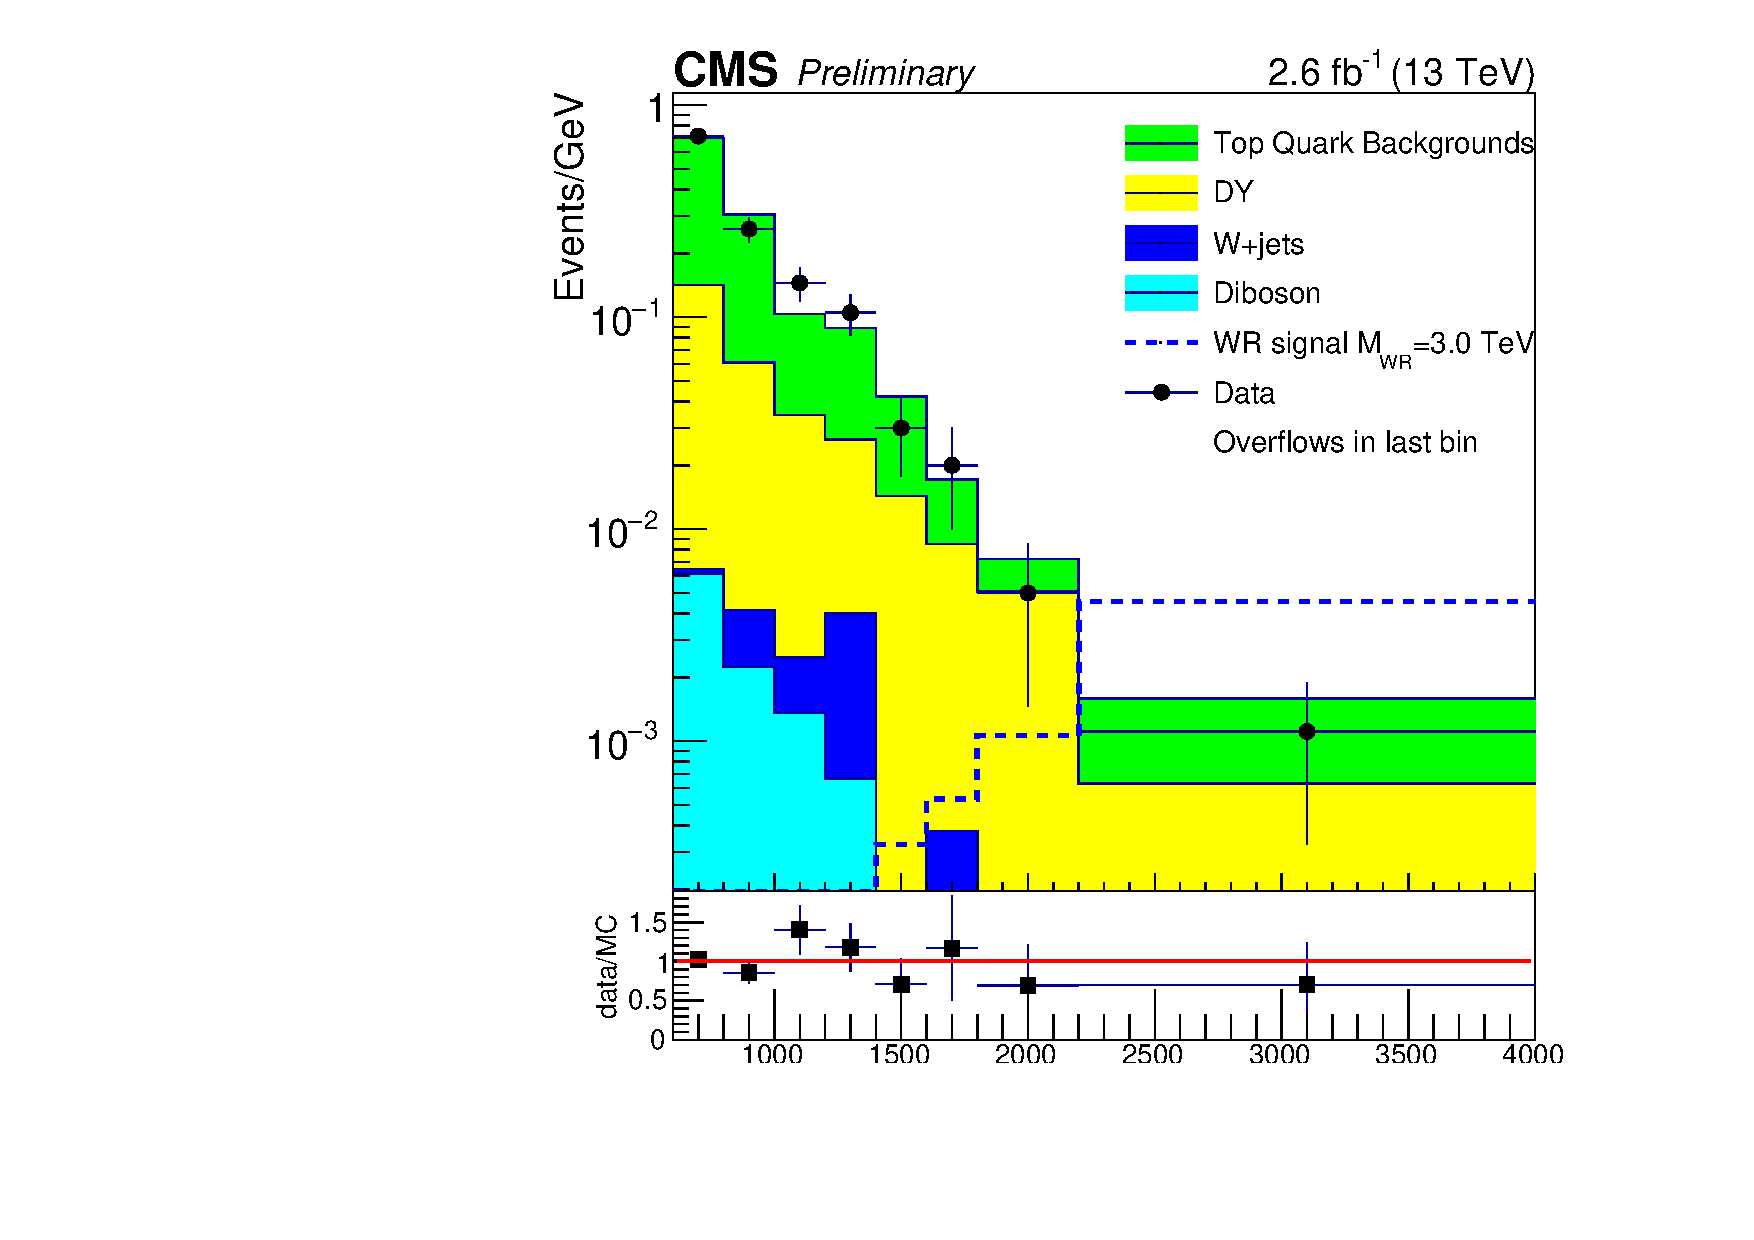
\includegraphics[width=0.65\textwidth]{figures/Mlljj_2012Bins_MWR3000Signal_SignalRegion_EEChannelBkgndMC_DYMadHTAndIncl_TTBarFromData_WithUnblindedData_withRatio_log.pdf}
	}
	\subfigure{
		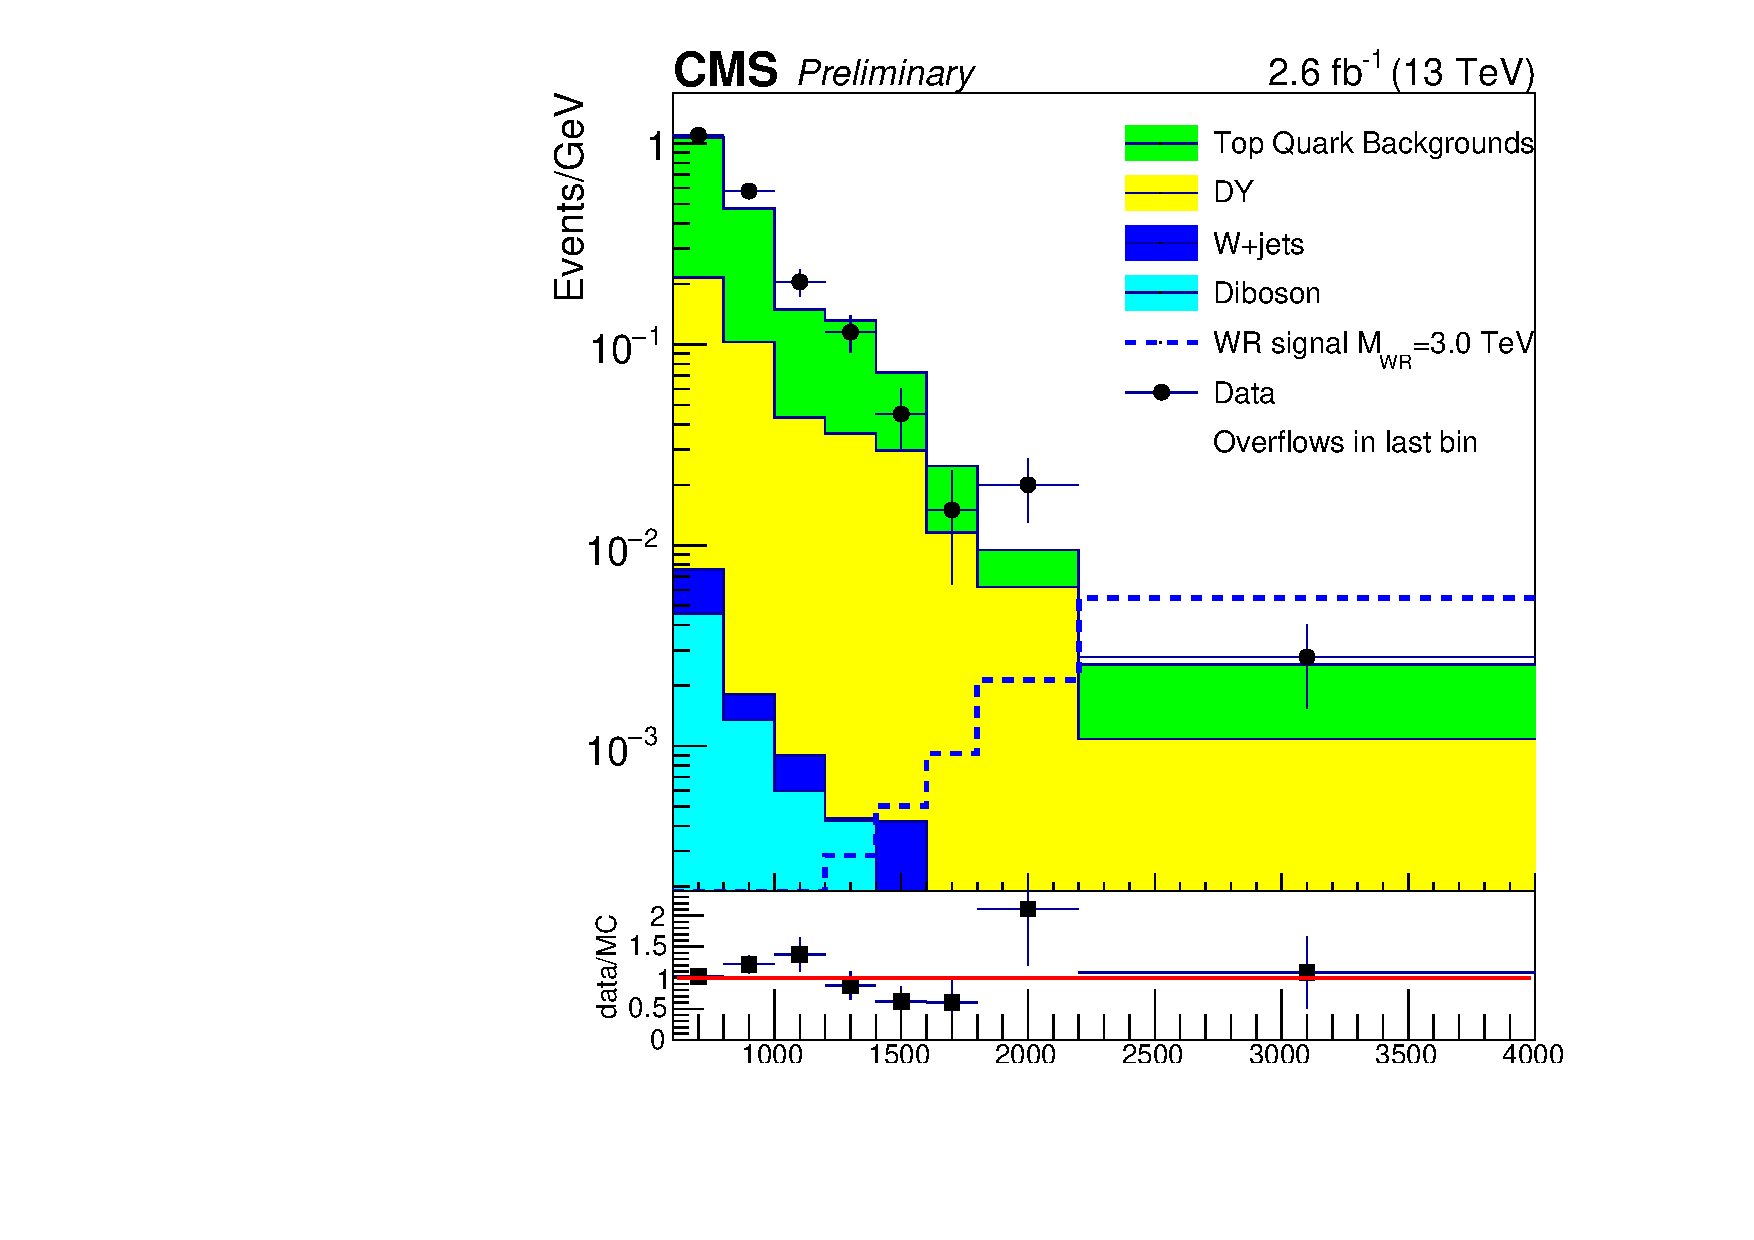
\includegraphics[width=0.65\textwidth]{figures/Mlljj_2012Bins_MWR3000Signal_SignalRegion_MuMuChannelBkgndMC_DYMadHTAndIncl_TTBarFromData_WithUnblindedData_withRatio_log.pdf}
	}
	\label{fig:obsAndExpMlljj}
	\caption{The $\Mlljj$ distributions after selections found in data, \WR simulations, and expected backgrounds.  The $ee$ ($\mu\mu$) 
		channel is shown on the left (right).}
\end{figure}

Upper limits on $\sigma(\WR) \times BR(\WR \rightarrow \ell\ell jj)$ were calculated at 95\% CL in each $\Mlljj$ window 
assuming $\mnul = \frac{1}{2}\mWR$.  Expected limits were calculated by setting the measured number of events $\Nlljj$ 
equal to the number of ST background events, and observed limits were calculated by setting $\Nlljj$ equal to the number 
of events found in data.  The expected and observed limits as functions of \mWR are shown in Figure \ref{fig:oneDimLimits}.  
Subsequently, the expected and observed cross section limits for $\mnul = \frac{1}{2}\mWR$ were extrapolated into \mnul 
and \mWR exclusion limits.

\begin{figure}[btp]
	\centering
	\subfigure{
		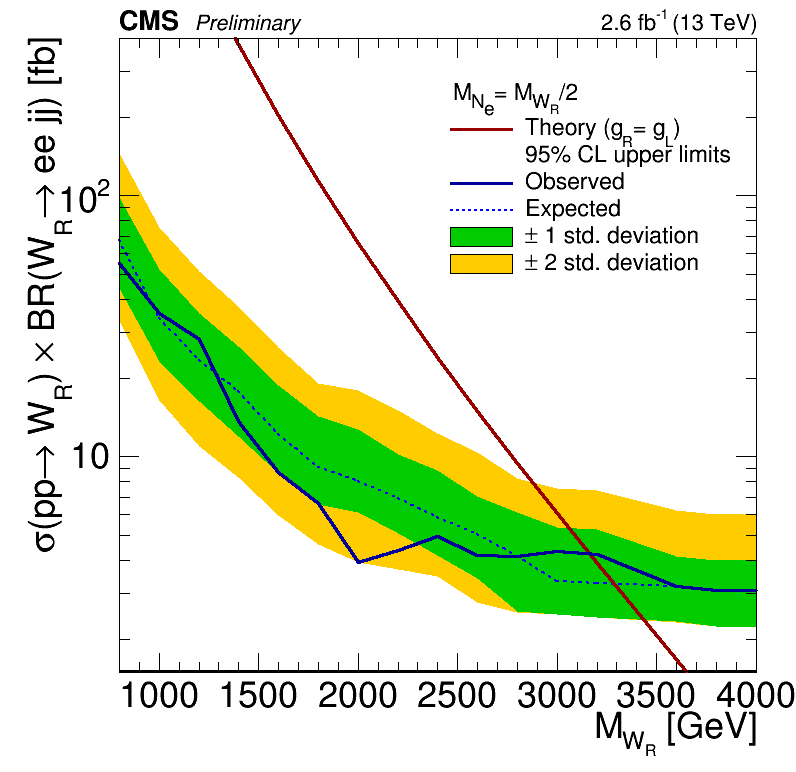
\includegraphics[width=0.65\textwidth]{figures/limWReejj_SHv19700toysAprilTwentyThree.png}
	}
	\subfigure{
		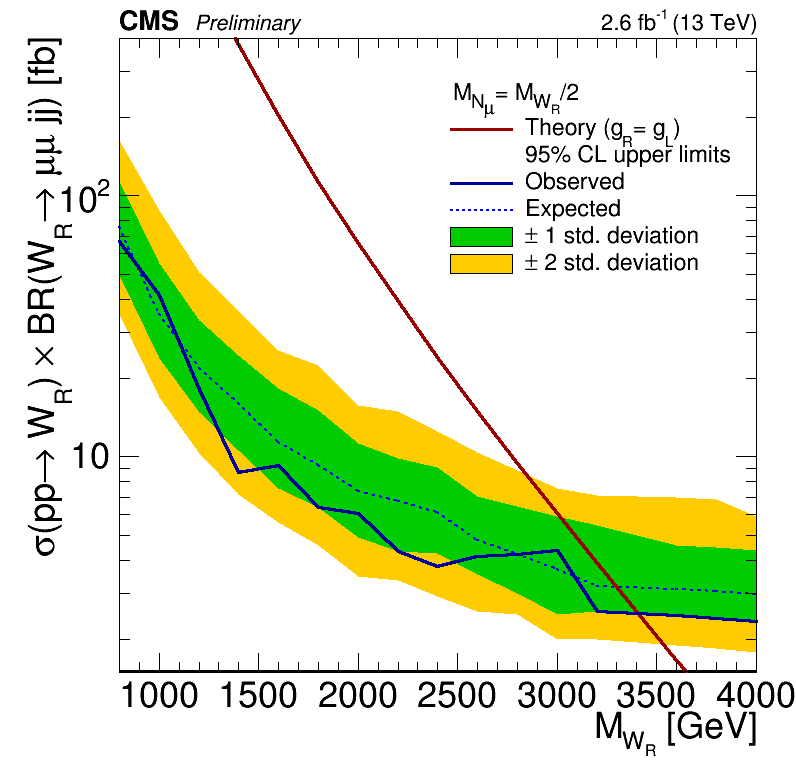
\includegraphics[width=0.65\textwidth]{figures/limWRmumujj_SHv19700toysAprilTwentyThree.png}
	}
	\label{fig:oneDimLimits}
	\caption{Limits on $\sigma(\WR) \times BR(\WR \rightarrow \ell\ell jj)$ at 95\% CL versus \mWR hypothesis.  The $ee$ ($\mu\mu$) channel 
	is shown on the left (right).}
\end{figure}

The limits on $\sigma(\WR) \times BR(\WR \rightarrow \ell\ell jj)$ for any \mnul were linearly proportional to the signal 
efficiency $\chi$ of the event selection multiplied by the \WR cross section $\sigma(\WR)$, $\chi \times \sigma(\WR)$.  
Since the estimated background was only sensitive to the \mWR hypothesis, the limits at two points with the same \mWR but 
different \mnul only differed by the ratio of $\chi \times \sigma(\WR)$ at the points.  Since the $\sigma(\WR) \times BR(\WR \rightarrow \ell\ell jj)$ 
limit was known at $(\mWR^{a}, \mnul^{a} = \frac{1}{2}\mWR^{a})$, the limit at any other point $(\mWR^{a}, \mnul^{b} \neq \frac{1}{2}\mWR^{a})$ 
could be calculated as:

\begin{equation}
	Limit[(\mWR^{a}, \mnul^{b} \neq \frac{1}{2}\mWR^{a})] = \frac{\chi[(\mWR^{a}, \mnul^{b} \neq \frac{1}{2}\mWR^{a})]}{\chi[(\mWR^{a}, \mnul^{a} = \frac{1}{2}\mWR^{a})]} \quad Limit[(\mWR^{a}, \mnul^{a} = \frac{1}{2}\mWR^{a})]
\label{eq:limitExtrapolation}
\end{equation}
The dependence of $\chi$ on \mnul and \mWR was estimated by simulating additional $\WR \rightarrow \ell\ell jj$ samples with 
\mWR increasing from 800 to 4000 $\GeV$ in 100 $\GeV$ steps.  At each \mWR value, at least 20 samples were produced with 
different \mnul values between 0 $\GeV$ and \mWR.  
%in steps of:
%\begin{itemize}
%	\item 25 $\GeV$ from 0 to 300 $\GeV$,
%	\item 100 $\GeV$ from 300 to $\mWR - 200$ $\GeV$,
%	\item 25 $\GeV$ from $\mWR - 200$ to \mWR $\GeV$
%\end{itemize}
%Smaller steps were used in regions where $\chi$ had a strong dependence on \mnul.
The standard full simulation and reconstruction used to produce \WR samples with $\mnul = \frac{1}{2}\mWR$ required enormous 
computational resources that were not available for the limit extrapolation procedure described here.  Instead, additional \WR 
simulations were produced using only the first simulation step.  \PYTHIA simulated the \WR production and decay into leptons 
and quarks, and the hadronization of quarks into jets.  Similar to reconstructed jets, jets from \PYTHIA were clustered from 
individual hadrons, leptons and photons in a cone of radius $\Delta R =$ 0.4.  After jet clustering, the offline selection was 
applied, excluding lepton and jet ID selections.  The efficiency of this selection $\chi^'$ was measured as a function of 
$(\mWR, \mnul)$, and used in place of $\chi$.  Then, $\chi^'$ and Equation \ref{eq:limitExtrapolation} were used to extrapolate 
the $\sigma(\WR) \times BR(\WR \rightarrow \ell\ell jj)$ limits calculated for $\mnul = \frac{1}{2}\mWR$ to new limits $L'$ for 
$\mnul \neq \frac{1}{2}\mWR$.  The resulting $\sigma(\WR) \times BR(\WR \rightarrow \ell\ell jj)$ limits were rescaled by $\sigma(\WR)$ 
for $\mnul \neq \frac{1}{2}\mWR$ to obtain the \mnul and \mWR exclusion limits at 95\% CL shown in Figure \ref{fig:twoDimLimits}.

\begin{figure}[tp]
  \centering
  
  \subfigure{
    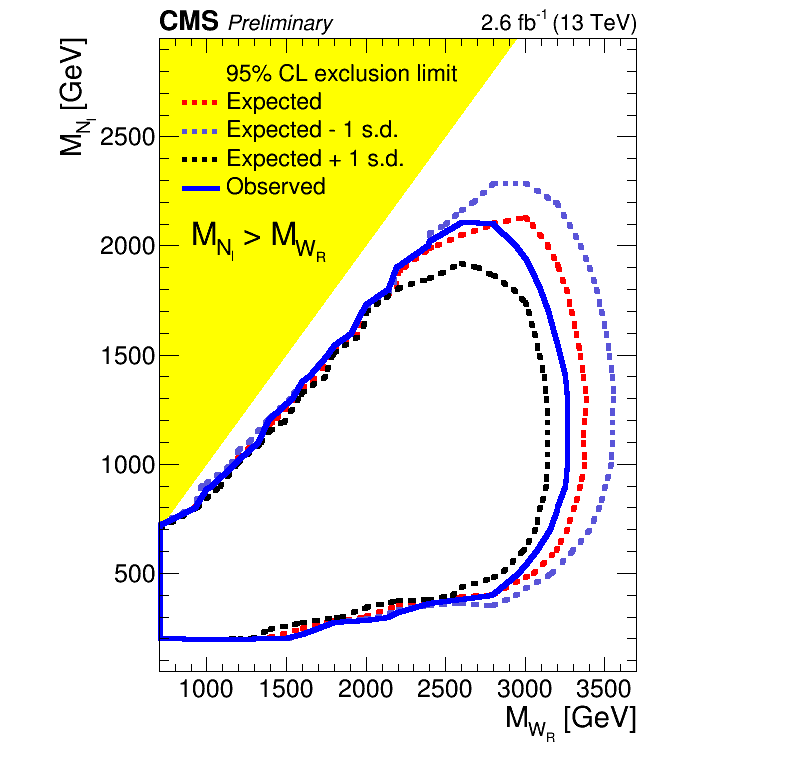
\includegraphics[width=0.65\textwidth]{figures/lim2dWReejj_SHv19700toysAprilTwentyThree_exclusionOverlayWithExpPlusMinusOneSigma.png}
  }
  \subfigure{
    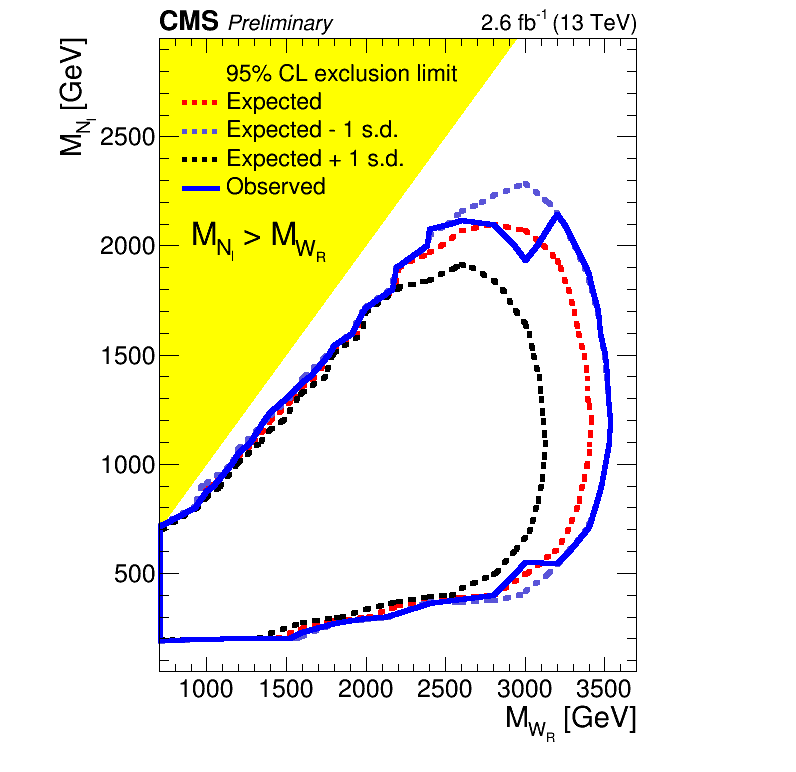
\includegraphics[width=0.65\textwidth]{figures/lim2dWRmumujj_SHv19700toysAprilTwentyThree_exclusionOverlayWithExpPlusMinusOneSigma.png}
  }
  \caption{The exclusion limits on \mWR and \mnul at 95\% CL for $\WR \rightarrow eejj$ (left) and $\WR \rightarrow \mu\mu jj$ (right).}
  \label{fig:twoDimLimits}
 
\end{figure}

The difference between the selection efficiencies $\chi^'$, without reconstruction, and $\chi$ was estimated by simulating 
$\WR \rightarrow \ell\ell jj$ at $\mWR =$ 2400 and 4000 $\GeV$ and several $\mnul \neq \frac{1}{2}\mWR$ with detector 
response simulations and particle reconstruction, and calculating limits with these events.  Simulated events were selected with the online and offline selection 
requirements, and the limits $L_{true}$ on $\sigma(\WR) \times BR(\WR \rightarrow \ell\ell jj)$ were calculated at each 
$(\mWR, \mnul \neq \frac{1}{2}\mWR)$ point.  For $\mnul \gtrsim \frac{1}{8}\mWR$, $L_{true}$ and $L'$ were consistent 
within their uncertainties.  For $\mnul \lesssim \frac{1}{8}\mWR$, the limit $L_{true}$ was stronger than $L'$ because of 
pileup jets.  $L_{true}$ was calculated using simulated events that included pileup interactions, on average 10 per event, that 
produced pileup jets, which enabled more \WR events to pass the full selection.  The resulting increase in signal selection 
efficiency $\chi$ extended the excluded \WR production region to lower \mnul values.  Although $\chi > \chi^'$ in this region, 
both signal selection efficiencies were below 10\%, and at every \mWR value the difference in the lowest excluded \mnul between 
$L_{true}$ and $L'$ was less than 100 $\GeV$.  The extrapolated limit $L'$ represented the result, and, since $L'$ was weaker 
than $L_{true}$, no correction was applied to it.

Using 2015 data \mWR production was excluded at 95\% CL for $\mWR \lesssim 3500 (3300) \GeV$ in the $\mu\mu$- ($ee$-) channel.  
The exclusion limits were consistent with ST expectations, and relative to the Run I limits, the mass limits in the $\mu\mu$- 
($ee$-) channel were extended 400 $\GeV$ (400 $\GeV$) higher in \mWR, and 150 $\GeV$ (300 $\GeV$) higher in \mnul.


%%%%%%%%%%%%%%%%%%%%%%%%%%%%%%%%%%%%%%%%%%%%%%%%%%%%%%%%%%%%%%%%%%%%%%%%%%%%%
